% !TEX root=../../mt-motion-analysis.tex
\chapter{Background - Deep learning}

\section{Machine learning - ELLER BARA DL??} \label{sec:ML}
A supervised machine learning problem can be described as finding a mapping between some input and output data, e.g. an image and a category, based on labeled input-output combinations. The idea with such methods is that a mapping found for the available data also should represent unseen data of the same type, i.e. it should generalize. To be able to get a measure of this generalization the available data is divided into two parts, training data and test data. The training data is used to find the mapping and the test data is used to evaluate how well it performs on unseen data \cite{Bishop2006}.

This chapter gives a brief introduction to a special type of machine learning called deep learning, which forms the basis of this work.

FIXAA DEN HAR SECTION INDELNINGEN...
\subsection{Deep Neural Networks}
\glspl{dnn} are combinations of linear and non-linear functions trained to approximate some other, potentially very complicated, function. The output of the network is formed as $f(x) = f_n(f_{n-1}(... f_1(f_0(x))))$ resulting in the layer terminology since the output from one function is passed as input to the subsequent one \cite{Goodfellow2016}.

 Below the layers functions used in our work are briefly explained.

\subsubsection{Dense layer}
The dense, or fully connected, layer is the basic model for a feedforward network. The outputs of such a layer is formed as linear combinations of the inputs and bias terms. Usually a non-linear activation function is applied to to this to be able to capture more general behaviors, resulting in the output

\begin{equation}
    y_i = h\Big( \sum_{j=1}^D w_{ij}x_j + b_i \Big).
    \label{eq:dense}
\end{equation}

$h(\cdot)$ is a non-linear activation. $x_j$, $j \in \{1, \hdots, D\}$ are the inputs to the layer, $w_{ij}$ and $b_i$ are the weights and biases learned during training \cite{Bishop2006}. A network with two dense layers is shown in Figure \ref{fig:dense}.

\begin{figure}
  \centering
  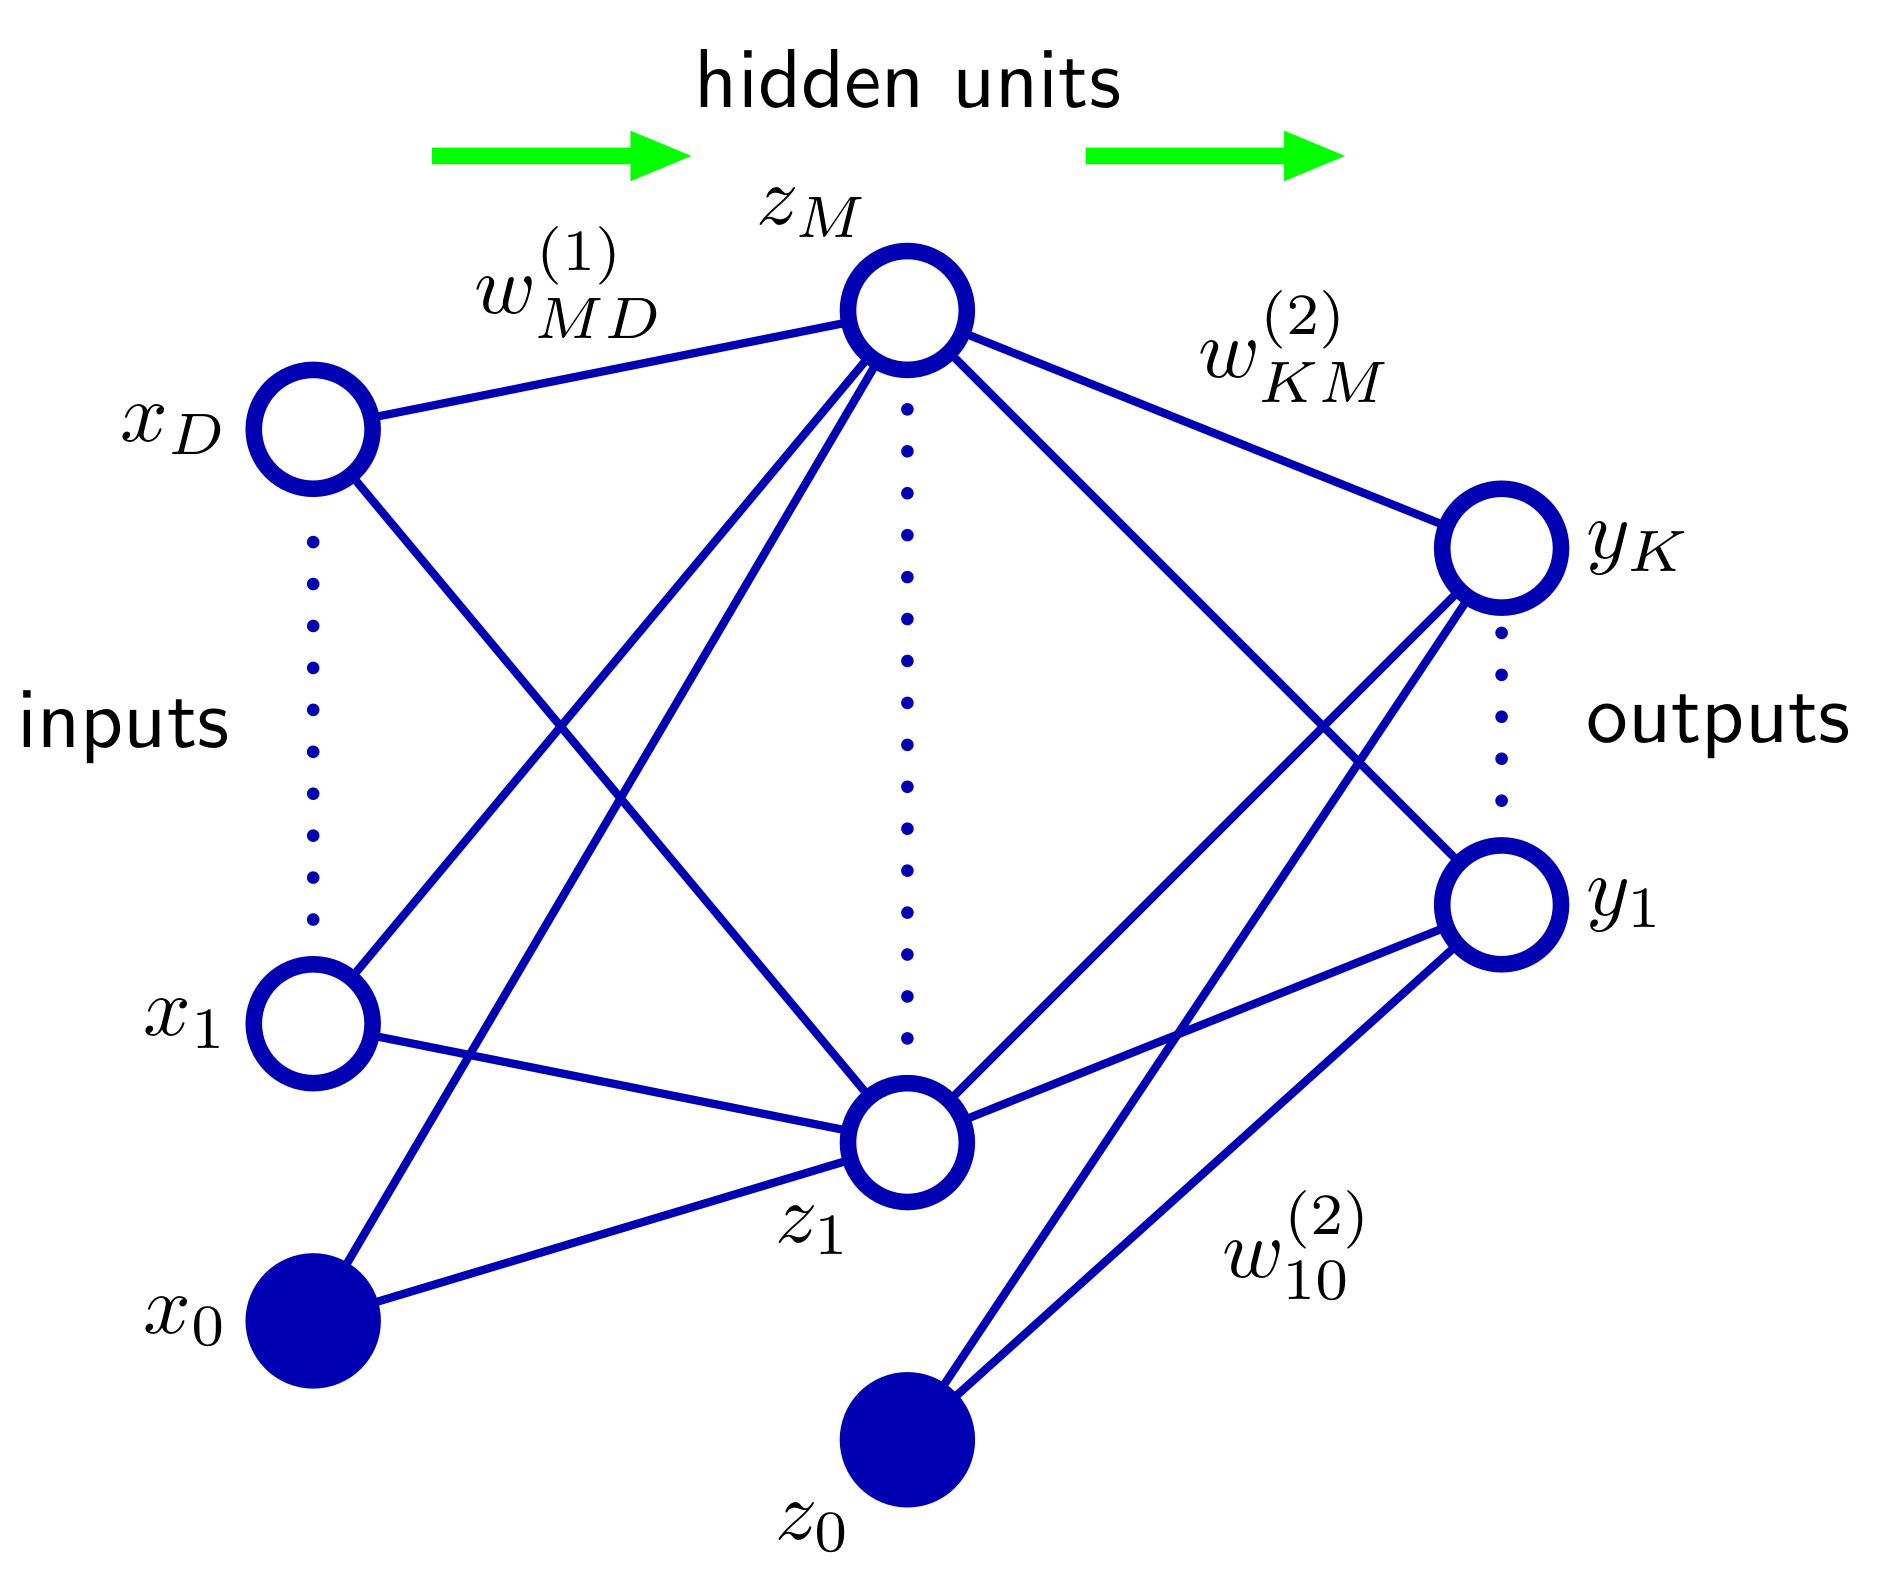
\includegraphics[width=0.5\textwidth]{files/figs/mlp.png}
  \caption{Feedforward neural network with two densely connected layers. Each line corresponds to one trainable parameter. $x_0$ and $z_0$ can be seen as ones added to the inputs introducing the bias terms \cite{Bishop2006}.}
  \label{fig:dense}
\end{figure}

\subsubsection{Convolutional layers}
Convolutional layers have proved successful for feature extraction from for instance time series or images. A reason for this is that they are equivariant to translation, meaning that patterns in a time series will be recognized in the same way no matter at which time steps they occur. The 1D convolution operation can be seen in \eqref{eq:conv}. When applied to for instance images it is performed in two dimensions.

\begin{equation}
   (x * w)(t) = \sum_{a=-\infty}^\infty x(a)w(t-a)
   \label{eq:conv}
\end{equation}

$x$ is the input and $w$ is the kernel or filter which consist of the trainable parameters. As the kernel size is not affected by the input size the convolutional layer can be applied to inputs of different size, which is not possible with for instance the fully connected layer \cite{Goodfellow2016}.

backprop, layers, optimizers

\subsection{Training of }
When training the network a loss function which describes the performance of the model is evaluated. The process of finding model parameters to minimize this function is referred to as training. For deep learning models

For a classification problem with $K$ mutually exclusive classes the categorical cross-entropy is commonly used. With this loss the labels are one-hot encoded meaning that each label is represented by $K$ binary variables, i.e. $y_i \in \mathbb{Z}_2^K$. Each variable represents a class and $y_i^{(k)} = 1$ for the $k$ corresponding to the class of the label and 0 otherwise. The final layer of the model has $K$ outputs with softmax activations. The loss to be minimized is shown in \eqref{eq:cat-cross-entr} \cite{Bishop2006}.

% $k \in \{1, \hdots, K \}$. Each variable represents a class and $y^{(k)} = 1$ for the $k$ corresponding to the class of the label and 0 otherwise. The final layer of the model has $K$ outputs and a softmax activation. The loss value is calculated as
\begin{equation}
    \mathcal{L}(\pmb{x}, \pmb{W}) = - \sum_{i=1}^N \sum_{k=1}^K y_i^{(k)} \log \hat{y}_i^{(k)}(x_i, \pmb{W}).
    \label{eq:cat-cross-entr}
\end{equation}

backprop



\subsubsection{activations osv, typ softmax, relu}



 %The convolution, $(x * w)(t)$, can be seen as a weighted average of some points around $x(t)$

\subsection{Historical background of deep learning} \label{sec:dl-history}
In 1943 McCulloch and Pitts \cite{McCulloch1943} presented a mathematical model of a neuron which at the time had limited capabilities (e.g. it did not learn), but lay the foundations for much of what today is considered to be deep learning. Ivakhnenko and Lapa \cite{Ivakhnenko1965} introduced what would later be called deep learning with the first multi-layered network in 1965. The first convolutional network was introduced by Fukushima in 1980 \cite{Fukushima1980}. A few years later, in 1989, LeCun et al. \cite{LeCun1989} showed it possible to train such networks with backpropagation. In 2009 Raina et al. \cite{Raina2009} suggested that \glspl{dnn} could efficiently be trained on \glspl{gpu}. Krizhevsky et al. \cite{Krizhevsky2012} used this when they with AlexNet proved it possible to train deeper networks which also greatly outperformed models of the time at computer vision tasks. Since then deep learning based methods has been adopted in various fields, such as computer vision, natural language processing, and even autonomous vehicles \cite{NazmusSaadat2020}.

\subsection{Explainability} \label{sec:explainability}
Much of the recent progress in the deep learning space is inherently incomprehensible for us humans, due to its black-box nature and the size of the models \cite{Du2018}. However, explainability is important at many stages of the development of an AI-system. When the systems performance is at sub-human levels it simplifies for human experts to improve it. When the system achieves similar results human experts it can help enforce trust to the system. Finally, in a scenario where the AI outperforms humans it can help us get a better understanding of the problem \cite{Selvaraju2016}. With these methods playing a bigger role in fields such as healthcare the importance of explainable decisions also grows from a legal and ethical perspective \cite{Amann2020}.

\subsubsection{Gradient-weighted Class Activation Mapping (Grad-CAM)} \label{sec:grad-cam}
Although most deep learning models are not interpretable there are post-hoc methods which tries to explain decisions. Selvaraju et al. \cite{Selvaraju2016} suggested one such method, called \gls{grad-cam}, where an activation map is calculated which shows what parts of the data is important for the decisions. Considering a neural network with convolutional layers as feature extractors followed by \gls{gap} and dense layers for classification \gls{grad-cam} is based on the final part of the network. Let $y_c$ be the output corresponding to class $c$ and $A$ be the final feature map of height $H$, width $W$, and with $F$ filters. The \gls{grad-cam} activation, $M_{GC}$, is then calculated as follows:

\begin{align}
 \begin{split}
  w_k^c &= \frac{1}{H \times W} \sum_{i=1}^H \sum_{j=1}^W \frac{\partial y_c}{\partial A_{ij}^k} \\
  M_{GC} &= ReLU \big ( \sum_{k=1}^F w_k^c A^k \big)
  \label{eq:grad-cam}
 \end{split}
\end{align}

The resulting activation map is importance values $\in \mathbb{R}^{H \times W}$. If the input is a time series this means that by designing the network to not alter the time dimension an importance value is obtained for each time step.

\subsection{Consistent Rank Logits (CORAL)}
Categorical data with a natural ordering are considered to be ordinal, examples of such data are the response to some medical treatment (e.g. poor, fair, good) \cite{Agresti2007} or the age of a person \cite{Cao2019}.

When classifying ordinal data it is desirable to exploit the fact that the categories are ordered \cite{Agresti2007}. An ordinal classification problem, or ordinal regression as it is also referred to, can be formulated as assigning labels, $y \in \mathcal{Y} = \{\mathcal{C}_0, \mathcal{C}_1, \hdots, \mathcal{C}_{K-1} \}$, to inputs $\pmb{x}$, where the classes $\mathcal{C}_0 \prec \mathcal{C}_1 \prec \hdots \prec \mathcal{C}_{K-1}$ according to some ordering relation \cite{Cao2019}.

Li and Lin \cite{Li2007} presented a method for ordinal regression where the combined result of $K-1$ binary classifiers for $K$ classes were used. Each classifier checked whether the rank of the sample class was larger than rank $r_k \in \{r_1, \hdots r_{K-1}\}$. Niu et al. \cite{Niu2016} developed this further using a multi-output \gls{cnn} as $K-1$ binary classifiers, called OR-CNN. The classifiers share all weights except the ones in the output layer. This method achieved \gls{sota} performance on datasets where age was estimated based on facial images. However, consistency was not guaranteed in the predictions, e.g. sometimes simultaneously predicting an age under 20 and over 30. Cao et al. \cite{Cao2019} addressed this issue with \gls{coral} which is an architecture-agnostic method that can extend any neural network based classifier. Similarly to OR-CNN \gls{coral} uses $K-1$ binary classifiers, here however sharing all weights parameters apart from the biases in the output layer. Instead of representing the labels as one-hot encodings they are now formed as $K-1$ binary labels, i.e. $y \in \mathbb{Z}_2^{K-1}$, where $y_i^{(k)} = 1$ if the the rank of the class is greater than $r_k$ and 0 otherwise. By minimizing the loss funtion By training the model with the loss function %The model is then trained with the loss function %together with a cost matrix, $\mathcal{C}_{y,r} = | y - r |$ penalizing the distance to the correct rank.

\begin{equation}
 \mathcal{L}(\pmb{W}, \pmb{b}) = - \sum_{i=1}^N \sum_{k=1}^{K-1} \lambda^{(k)} [\log(\sigma(g(\pmb{x}_i, \pmb{W}) + b_k))y_i^{(k)} + \log(1 - \sigma(g(\pmb{x}_i, \pmb{W}) + b_k))(1 - y_i^{(k)})],
 \label{eq:coral-loss}
\end{equation}

\begin{conditions}
 $$\pmb{W}$$               & = & all model parameters except biases of final layer \\
 $$\pmb{b}$$               & = & bias weights of final layer \\
 $$\lambda^{(k)}$$         & = & loss weight for class $k$ \\
 $$g(\pmb{x}_i, \pmb{W})$$ & = & output of penultimate layer \\
 $$\sigma(z)$$             & = & logistic sigmoid function, $1/(1 + \exp(-z))$ \\
 $$\sigma(g(\pmb{x}_i, \pmb{W}) + b_k)$$ & = & predicted output of binary classifier $k$
\end{conditions}

it can be shown that

\begin{equation}
 b_1 \geq b_2 \geq \hdots \geq b_{K-1}.
\end{equation}

The proof can be found in \cite{Cao2019} and from this and the shared weights it follows that

% \begin{equation}
%  \widehat{P} \big( y_i^{(1)} = 1 \big) \geq \widehat{P} \big( y_i^{(2)} = 1 \big) \geq \hdots \geq \widehat{P} \big( y_i^{(K-1)} = 1 \big)
% \end{equation}
\begin{equation}
 \widehat{P} \big( y_i > r_1 \big) \geq \widehat{P} \big( y_i > r_2 \big) \geq \hdots \geq \widehat{P} \big( y_i > r_{K-1} \big)
\end{equation}

since the only thing that differs between the predictions is the bias. The probabilities for the individual classes are computed from this as

% since the only thing that differs between the predictions is the bias. Note that $\widehat{P}(y_i > r_k)$ is the predicted probability that the rank of $y_i$ is greater than $k$. The probabilities for the individual classes are computed from this as

% \begin{alignat}{2}
%   % \begin{split}
%   &\widehat{P}\big(\mathcal{C}_0 \big) &&= 1 - \widehat{P}\big(y_i > r_1\big) \\
%   &\widehat{P}\big(\mathcal{C}_1 \big) &&= \widehat{P}\big(y_i > r_1\big) - \widehat{P}\big(y_i > r_2\big) \\
%   & && \vdots \\
%   &\widehat{P}\big(\mathcal{C}_{K-1} \big) &&= \widehat{P}\big(y_i > r_{K-1}\big)
% % \end{split}
% \end{alignat}

\begin{equation}
  \begin{alignedat}{2}
    &\widehat{P}\big(\mathcal{C}_0 \big) &&= 1 - \widehat{P}\big(y_i > r_1\big) \\
    &\widehat{P}\big(\mathcal{C}_1 \big) &&= \widehat{P}\big(y_i > r_1\big) - \widehat{P}\big(y_i > r_2\big) \\
    & &&\vdots \\
    &\widehat{P}\big(\mathcal{C}_{K-1} \big) &&= \widehat{P}\big(y_i > r_{K-1}\big).
  \end{alignedat}
\end{equation}

% \begin{align}
%     \begin{split}
%       &&\widehat{P}\big(\mathcal{C}_0 \big) &= 1 - \widehat{P}\big(y_i > r_1\big) \\
%       &&\widehat{P}\big(\mathcal{C}_1 \big) &= \widehat{P}\big(y_i > r_1\big) - \widehat{P}\big(y_i > r_2\big) \\
%       &\vdots \\
%       &&\widehat{P}\big(\mathcal{C}_{K-1} \big) &= \widehat{P}\big(y_i > r_{K-1}\big)
%     \end{split}
% \end{align}

% \begin{alignat}{2}
%   \begin{split}
%     \widehat{P}&\big(\mathcal{C}_0 \big) & = 1 - \widehat{P}\big(y_i > r_1\big) \\
%     \widehat{P}&\big(\mathcal{C}_1 \big) & = \widehat{P}\big(y_i > r_1\big) - \widehat{P}\big(y_i > r_2\big) \\
%     & & \vdots \\
%     \widehat{P}&\big(\mathcal{C}_{K-1} \big) & = \widehat{P}\big(y_i > r_{K-1}\big)
%   \end{split}
% \end{alignat}
% \begin{equation}
%     \begin{alignedat}{2}
%       &\widehat{P}\big(\mathcal{C}_0 \big) = 1 - \widehat{P}\big(y_i > r_1\big) \\
%       &\widehat{P}\big(\mathcal{C}_1 \big) &&= \widehat{P}\big(y_i > r_1\big) - \widehat{P}\big(y_i > r_2\big) \\
%       & &&\vdots \\
%       &\widehat{P}\big(\mathcal{C}_{K-1} \big) &= \widehat{P}\big(y_i > r_{K-1}\big)
%     \end{alignedat}
% \end{equation}
%The emergence of computing power discussed in Section \ref{sec:ML} allowing deeper networks shown by AlexNet \cite{Krizhevsky2012} blabla
